% Appendix A

\appendix
\renewcommand{\thechapter}{A}
\chapter{SIGMUND, manual de uso} % Main appendix title

\label{APP_SIGMUNDMAN} % For referencing this appendix elsewhere, use \ref{AppendixA}

\section{Introducción}

La aplicación \texttt{SIGMUND} permite llevar a cabo simulaciones del modelo dinámico descrito en el capítulo \ref{chapterDINAMICA}, tanto de forma interactiva como en modo \texttt{batch}.

El \textit{software} se ha desarrollado en \texttt{Python} y puede ejecutarse en cualquier entorno que disponga de la versión \texttt{3.0} o superior. Se recomienda instalar una distribución que incluya todos los paquetes habituales en cálculo científico. En concreto, la distribución \href{https://www.continuum.io/}{Anaconda} proporciona un entorno completo sobre el que instalar \texttt{SIGMUND} sin necesidad de añadir manualmente ningún paquete adicional.

El paquete se instala desde \texttt{github} clonando el repositorio:

\fontsize{3.5mm}{3.5mm}\selectfont
\begin{verbatim}
 clone https://github.com/jgalgarra/sigmund 
\end{verbatim}
\normalsize
%
%Este manual describe la aplicación en su versión \texttt{2.05}.
 
\section{Formato de los ficheros de entrada}
\label{sec:ASIGMUNDMAN_input_file_format}

Las simulaciones requieren dos ficheros de entrada para cada red, que se almacenan en el directorio \path{sigmund/src/pak_tfm/input}. El primero se llamará \texttt{XXX\_a.txt} donde \textit{XXX} puede ser cualquier nombre, lo único obligatorio es que termine en \texttt{\_a.txt}. El segundo debe llamarse \texttt{\_b.txt}. Por motivos de simplicidad, la interfaz de usuario se refiere a plantas y polinizadores, pero puede usarse para otros tipos de red mutualista.
El primer fichero contiene los coeficientes de la matriz de adyacencia en el sentido polinizador - planta, esto es, el beneficio mutualista que la presencia de cada individuo del polinizador $i$ supone para la planta $j$. Los datos se organizan en columnas, cada una de ellas correspondiente a una especie de planta, en modo texto y separados por tabuladores. Hay una fila por cada especie de polinizador y cinco adicionales con la población inicial de la especie de planta, el coeficiente $c_{j}$ (fórmula \ref{eq:alphavariable}), el término de fricción intraespecífica $\alpha_{j}$ y las tasas vegetativas de nacimiento y muerte.

En el fichero \texttt{\_b} se almacena la información en el sentido planta - polinizador, con tantas columnas como especies de estos segundos haya.

\begin{figure}[h!]
\centering
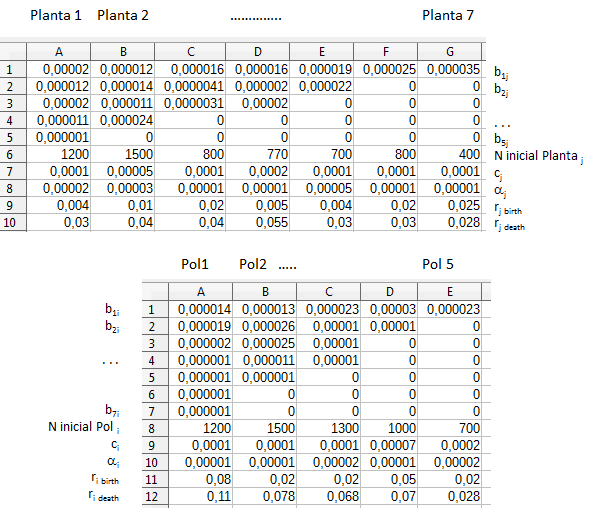
\includegraphics[scale=1]{ManFigs/matricessim.png}
\caption{Ejemplo de ficheros de entrada para la simulación de la figura \ref{fig:DINAMICA_SAT_exper_resilience_strong}.}
\label{fig:ASIGMUNDMAN_matricessim}
\end{figure}

\clearpage
\section{Uso interactivo}
\label{sec:ASIGMUNDMAN_ui}

$SIGMUND$ queda preparado para funcionar una vez clonado el repositorio. Navegar hasta el directorio \path{sigmund/src/pak_tfm} que se habrá creado en ese proceso. Si se utiliza \texttt{Windows} hágase doble click con el botón izquierdo sobre el icono \texttt{sigmund\_tool.py}. Bajo \texttt{Linux} se puede lanzar con el comando \texttt{sigmund\_tool.py}.

Aparecerán dos ventanas, una con la salida de la sesión \texttt{Python} y otra con la interfaz de usuario de \texttt{SIGMUND}. La primera puede redirigirse a un fichero o hacia donde el usuario considere conveniente.


\begin{figure}[h!]
\centering
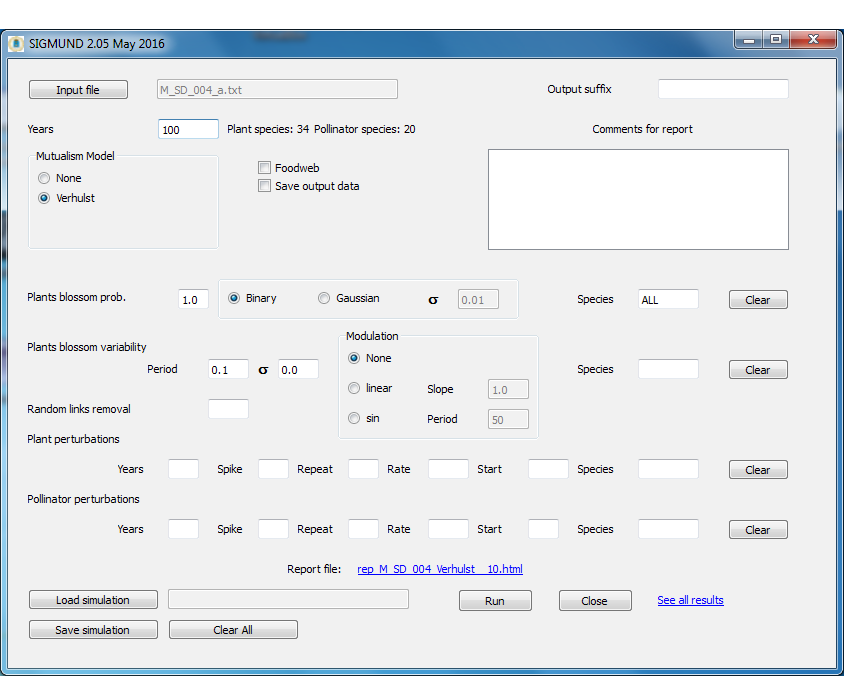
\includegraphics[scale=1]{ManFigs/sigmund_ui.png}
\caption{Interfaz de usuario de \texttt{SIGMUND} }
\label{fig:ASIGMUNDMAN_matricessim}
\end{figure}

La interfaz de usuario está construida con el entorno gráfico \texttt{Qt} por lo que la apariencia puede variar ligeramente dependiendo del sistema operativo y del juego de fuentes instalado. Este es el significado de los campos de entrada:

\begin{itemize}
\item \texttt{Input File}: nombre de cualquiera de los ficheros de configuración de la red almacenados en \path{./input}. Se puede escoger de forma manual o se cargará automáticamente si se recrea una simulación almacenada. La interfaz de usuario mostrará el número de especies de cada clase.

\item \texttt{Years}:  Duración de la simulación en años, obligatorio.

\item \texttt{Output suffix}: sufijo de salida opcional que se añadirá al nombre de los ficheros de salida que se escriben en  \path{./output}.

\item \texttt{Comments}: campo opcional de escritura libre que sirve, por ejemplo, para que una descripción del experimento se pueda guardar en el informe de ejecución.

\item \texttt{Mutualism Model}: indica si se usa el modelo de Verhulst modificado o no hay mutualismo.

\item \texttt{Food web}: indica si hay una \textit{food web} sobre la comunidad mutualista.

\item \texttt{Save output data}: indica si se quieren guardar los resultados numéricos de la simulación en ficheros de texto. Debido a que la simulación se calcula día a día, el tamaño de estos ficheros puede ser muy grande y se ralentizará la simulación.

\end{itemize}

El sistema puede atacarse de manera opcional con distintos tipos de perturbaciones:
\begin{itemize}
\item \texttt{Random links removal}: porcentaje de enlaces de la red que se retiran de manera aleatoria.

\item \texttt{Plants blossom probability}: Probabilidad de florecimiento. 

\begin{itemize}
	\item \texttt{Binary}: la floración de cada año se trata como un experimento de Bernouilli. Las especies indicadas en la lista florecen con la intensidad habitual o no lo hacen en absoluto.

    \item \texttt{Gaussian}: se modula la intensidad con una normal de media igual al parámetro de probabilidad y desviación estándar igual a $\sigma$.
    
    \item \texttt{Species}: lista de especies afectadas que puede ser un rango con formato \texttt{Python}, por ejemplo 1:3, una lista de números separados por comas o una combinación de ambos. El valor \texttt{ALL} indica que todas las especies sufren la perturbación.
\end{itemize}

\item \texttt{Plants blossom variability}: Variabilidad de la floración debida a la falta de coincidencia en el tiempo de la floración con la actividad animal.
\begin{itemize}
	\item \texttt{Period}: Fracción del año en que coinciden floración y actividad animal, modelada según una gaussiana.

    \item \texttt{Deviation}: Desviación estándar del periodo de floración.
    
    \item \texttt{Type}:  \texttt{None} desviación constante, \texttt{linear} desviación variable definida por la pendiente o \texttt{sinusoidal}, desviación variable modulada por una sinusoide del periodo especificado.
    
    \item \texttt{Species}: lista de especies afectadas.
\end{itemize}

\end{itemize}

Perturbaciones externas. Ataques exógenos (sequías, migraciones...) que pueden producir un aumento abrupto de las tasas
de mortalidad. Hay dos líneas de entrada, una para plantas y otra para animales.

\begin{itemize}
 \item \texttt{Years}: Duración de la perturbación en años.
 \item \texttt{Spike}: Fracción activa del periodo de perturbación. Útil en caso de perturbación repetitiva.
 \item \texttt{Spike}: Aumento de la tasa de mortalidad expresado en fracción unitaria.
 \item \texttt{Start}: Año de la simulación en que la perturbación empieza a tener efecto.
 \item \texttt{Species}: lista de especies afectadas.
\end{itemize}

Por último, los parámetros de una simulación pueden salvarse en un fichero y recuperarse posteriormente con:
\begin{itemize}
 \item \texttt{Load simulation}
 \item \texttt{Save simulation}
\end{itemize}

\subsection{Ejemplos}

En esta sección se presentan distintos casos de uso con el simulador y su significado ecológico.

\begin{figure}[h!]
\centering
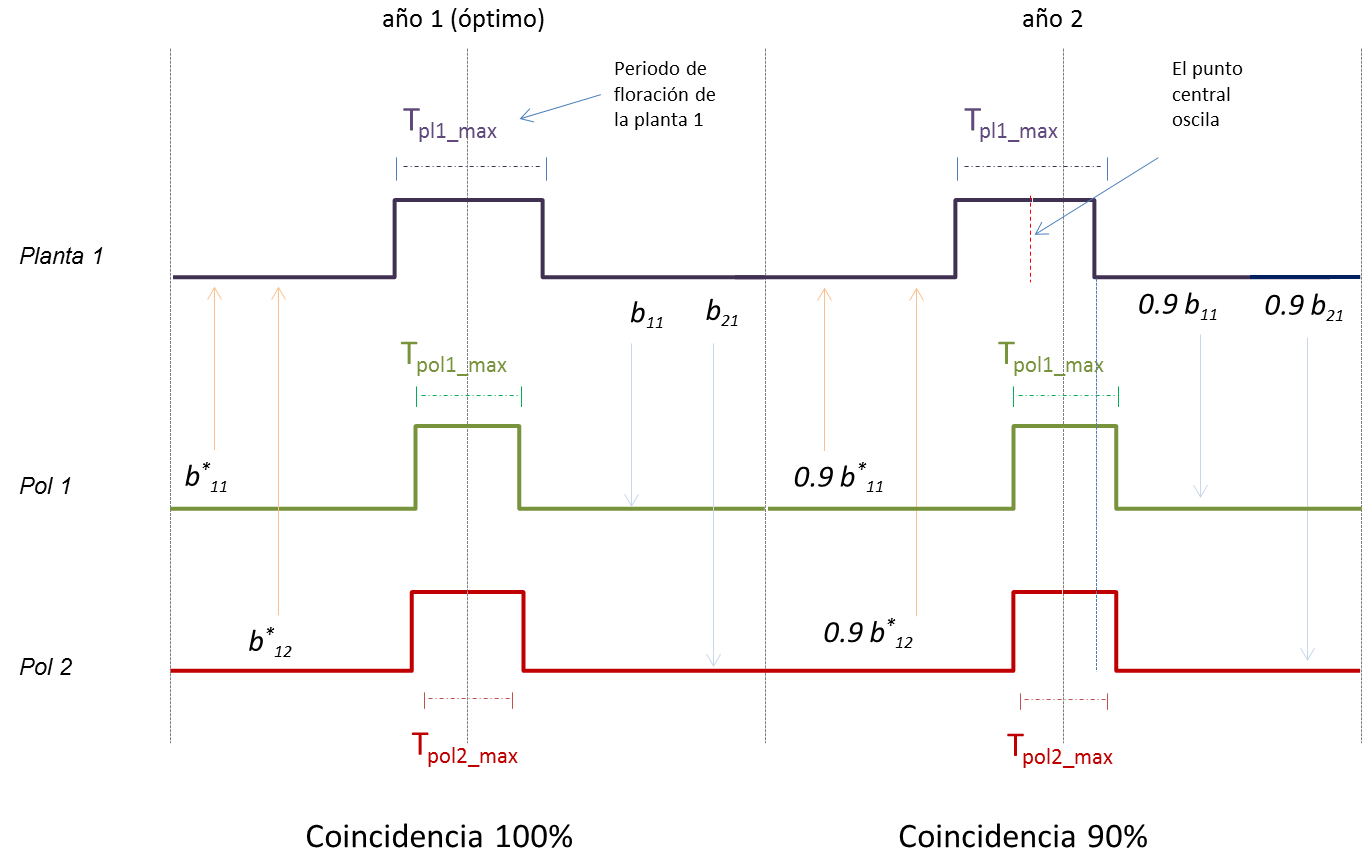
\includegraphics[scale=1]{ManFigs/sigmund_tiempos.png}
\caption{Significado de la coincidencia del periodo de floración}
\label{fig:ASIGMUNDMAN_sigmund_tiempos}
\end{figure}

En la figura \ref{fig:ASIGMUNDMAN_sigmund_tiempos} se ha representado el modelo simplificado que se emplea para el periodo de floración. El primer año el periodo de floración de las
plantas y de los animales coincide al $100\%$ con el de actividad de estos últimos, el beneficio mutualista es óptimo y los coeficientes planta polinizador son los que se leen de la
matriz de interacción. El segundo año, el periodo de floración se ha adelantado y el área de coincidencia es solo el $90\%$ del óptimo de manera que los coeficientes se multiplicarán por este factor reductor en la simulación.

\begin{figure}[h!]
\centering
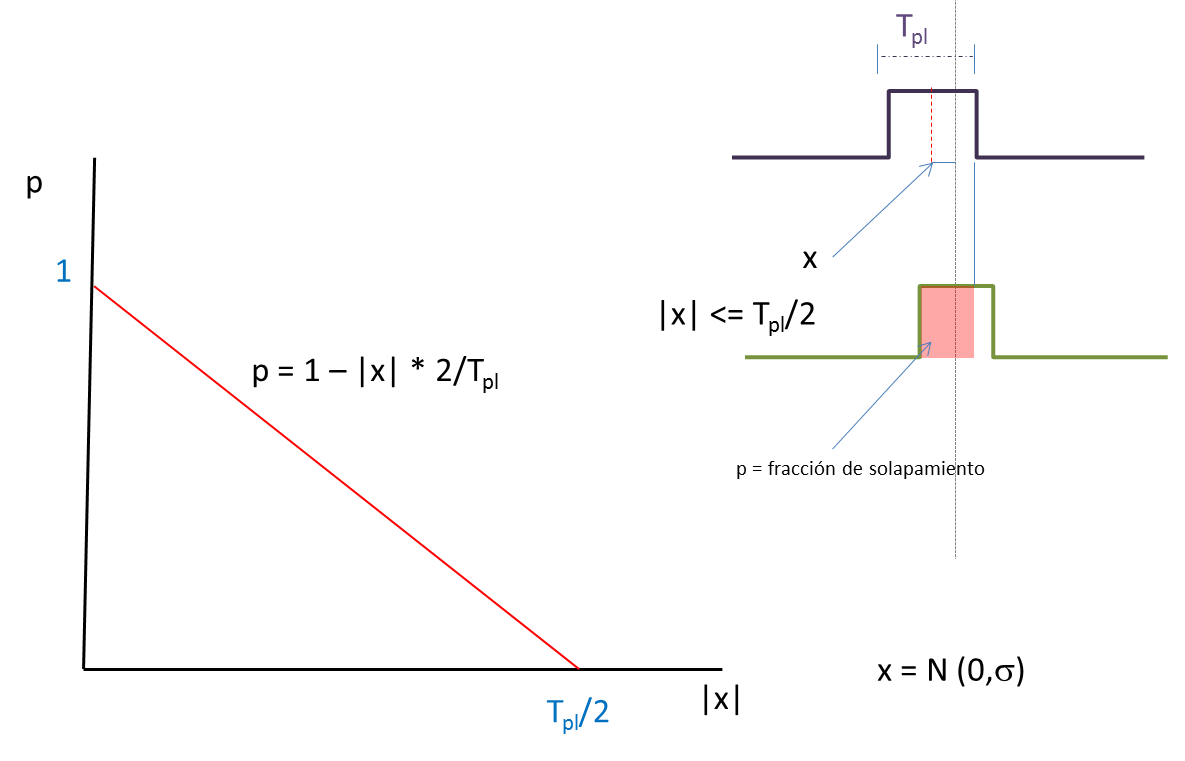
\includegraphics[scale=1]{ManFigs/sigmund_pendiente.png}
\caption{Cálculo del factor de multiplicación anual.}
\label{fig:ASIGMUNDMAN_sigmund_pendiente}
\end{figure}

El cálculo del factor $p$ por el que se multiplican los coeficientes mutualistas cada año, en función de la variabilidad, se representa en la figura \ref{fig:ASIGMUNDMAN_sigmund_pendiente}. Supongamos el caso más simple, en el que el valor medio de la variabilidad es constante. El periodo de coincidencia de la floración y la actividad animal $T_{pl}$ se ha introducido por la interfaz de usuario expresado como fracción del año, por ejemplo $0.1$. Si la floración se adelanta más de $0.05$ o se retrasa más de $0.05$ respecto del punto central óptimo no habría coincidencia y se multiplicaría por cero. Si está en ese rango, el factor multiplicativo $p$ se modela linealmente:

\begin{equation}
p = 1 - \frac{2|x|}{T_{pl}}
\label{eq:sigmund_p}
\end{equation}

Donde $x$ representa el desplazamiento del centro del periodo de floración. Si es igual a $0$, la situación es óptima y el factor $p$ vale $1$, si es mayor en valor absoluto que $1/2$ el valor $p$ es cero como se ha indicado y si está en un valor intermedio, el factor valdrá entre $0$ y $1$.

La variación anual del momento inicial de la floración se calcula, en el caso de media constante como una variable normal de media $0$ y desviación estándar $\sigma$. Si el valor de la desviación es pequeño frente al del periodo tendrá poco efecto, pero a partir de una relación $1$ a $10$ empieza a causar problemas notables.

El simulador ofrece dos posibilidades más. La primera de ellas es el crecimiento lineal de la desviación estándar a lo largo del periodo de estudio. De esta forma se puede estudiar el impacto de un aumento de la variabilidad a largo plazo inducido por cambio climático o por otras causas. La segunda es simular una variación cíclica modulando la desviación estándar por una sinusoide.

\begin{figure}[h!]
\centering
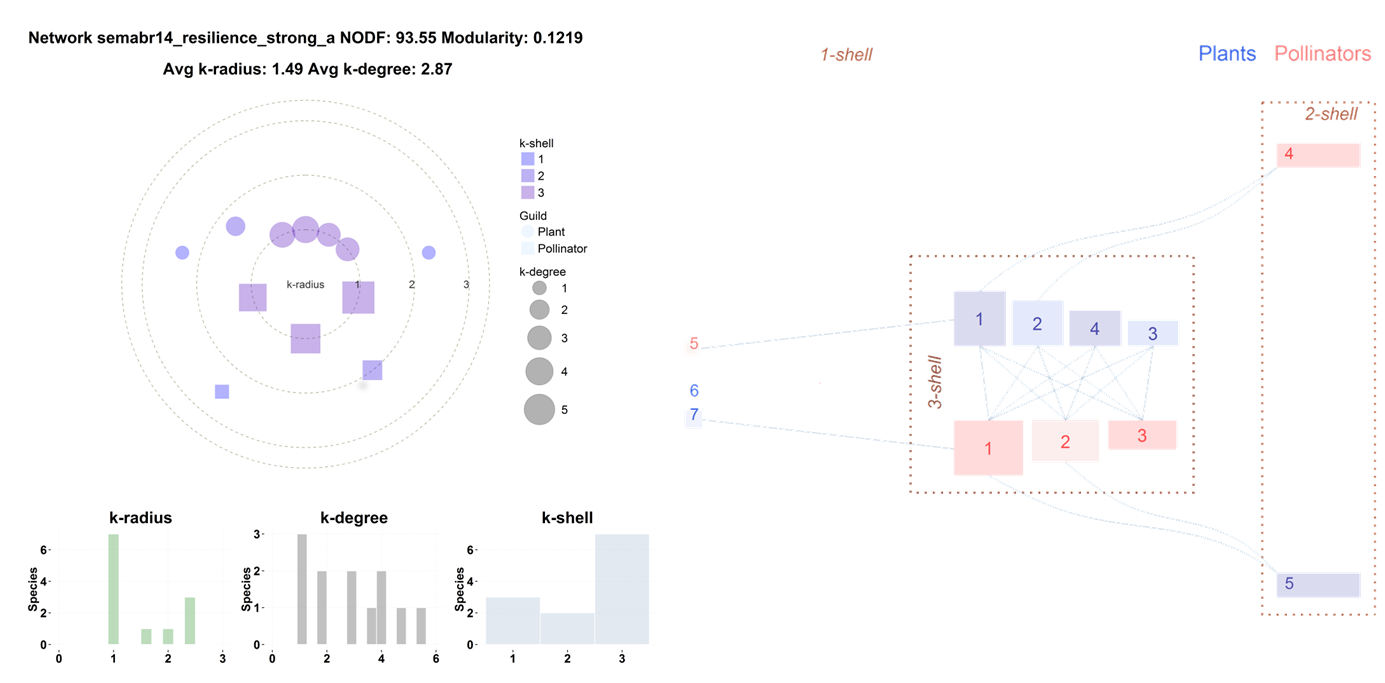
\includegraphics[scale=1]{ManFigs/sigmund_oscilacion_diag_red.png}
\caption{Diagrama polar y zigurta de la red ejemplo.}
\label{fig:ASIGMUNDMAN_sigmund_oscilacion_diag_red}
\end{figure}

Para los ejemplos, se analizará la dinámica de una pequeña red ficticia \ref{fig:ASIGMUNDMAN_sigmund_oscilacion_diag_red} que se usó en el capítulo \ref{chapterDINAMICA} y que allí se representó con el diagrama bipartito de la figura \ref{fig:DINAMICA_SAT_red_exper_resilience_strong}

\begin{figure}[h!]
\centering
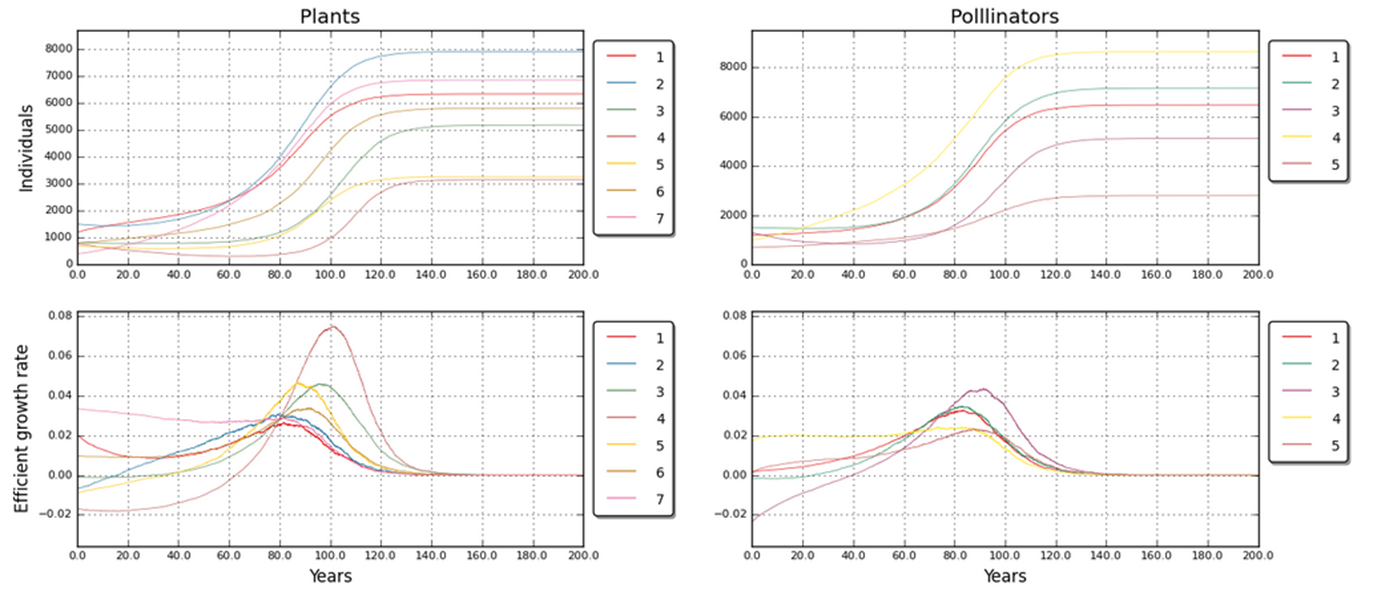
\includegraphics[scale=1]{ManFigs/sigmund_red_exper.png}
\caption{Evolución dinámica sin perturbaciones en la red ejemplo.}
\label{fig:ASIGMUNDMAN_sigmund_red_exper}
\end{figure}

\begin{figure}[h!]
\centering
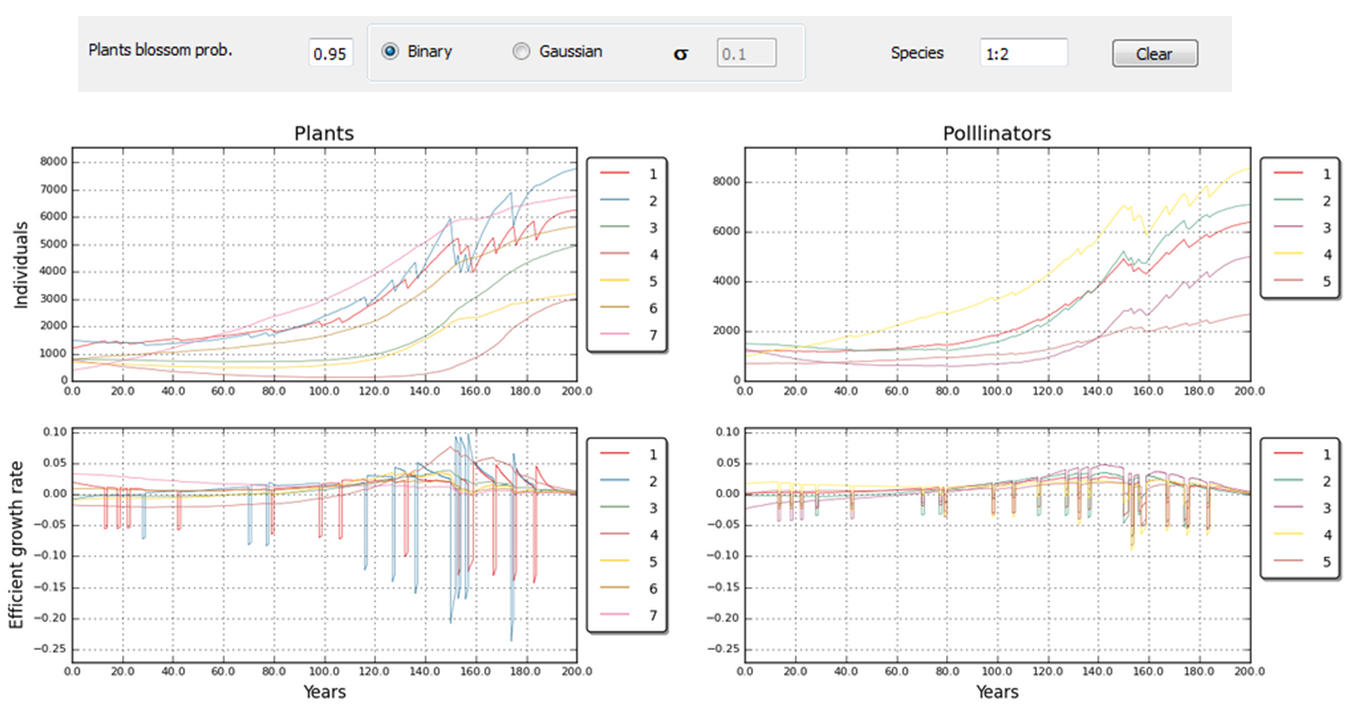
\includegraphics[scale=1]{ManFigs/sigmund_oscilacion_intensidad.png}
\caption{Perturbación binaria de la intensidad de floración.}
\label{fig:ASIGMUNDMAN_sigmund_oscilacion_intensidad}
\end{figure}

En la figura \ref{fig:ASIGMUNDMAN_sigmund_red_exper} se ve la evolución de las poblaciones del sistema. Puede comprobarse cómo el número de individuos de todas las especies crece hasta alcanzar el punto de equilibrio de poblaciones máximas en ausencia de perturbaciones. 

En la figura \ref{fig:ASIGMUNDMAN_sigmund_oscilacion_intensidad} se incluye una variación de la intensidad de la floración en las dos especies de planta más generalistas, la $1$ y la $2$. El tipo de perturbación es binaria y la probabilidad es $0.95$, así que, por término medio, el $95\%$ de los años la floración es normal y el $5\%$, inexistente. Se ve la caída abrupta de las tasas
de crecimiento eficiente de ambas especies de plantas cuando ocurre uno de estos eventos. Esto afecta a los polinizadores y en conjunto el sistema tarda más tiempo en alcanzar las poblaciones máximas.

\begin{figure}[h!]
\centering
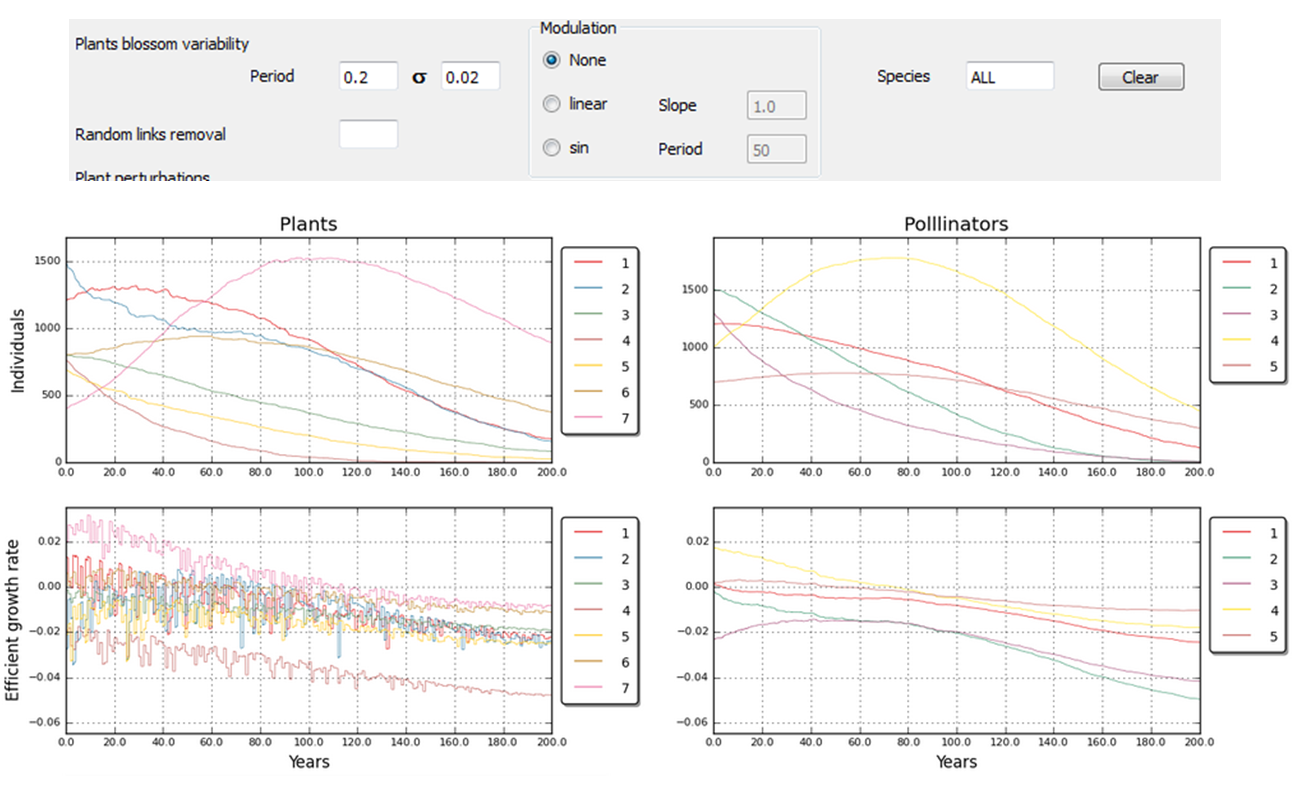
\includegraphics[scale=1]{ManFigs/sigmund_oscilacion_tiempo_none.png}
\caption{Perturbación gaussiana en el periodo de floración con desviación estándar constante.}
\label{fig:ASIGMUNDMAN_sigmund_oscilacion_tiempo_none}
\end{figure}

En la figura \ref{fig:ASIGMUNDMAN_sigmund_oscilacion_tiempo_none} se ha introducido una perturbación en el periodo de floración de todas las especies. Es una gaussiana de media $0.2$ y desviación estándar $0.02$. El valor se toma al inicio de cada año y se multiplica por los coeficientes de beneficio mutualista de las especies afectadas, todas las vegetales en este ejemplo. El efecto sobre el sistema global resulta devastador, la red se destruye.

\begin{figure}[hp!]
\centering
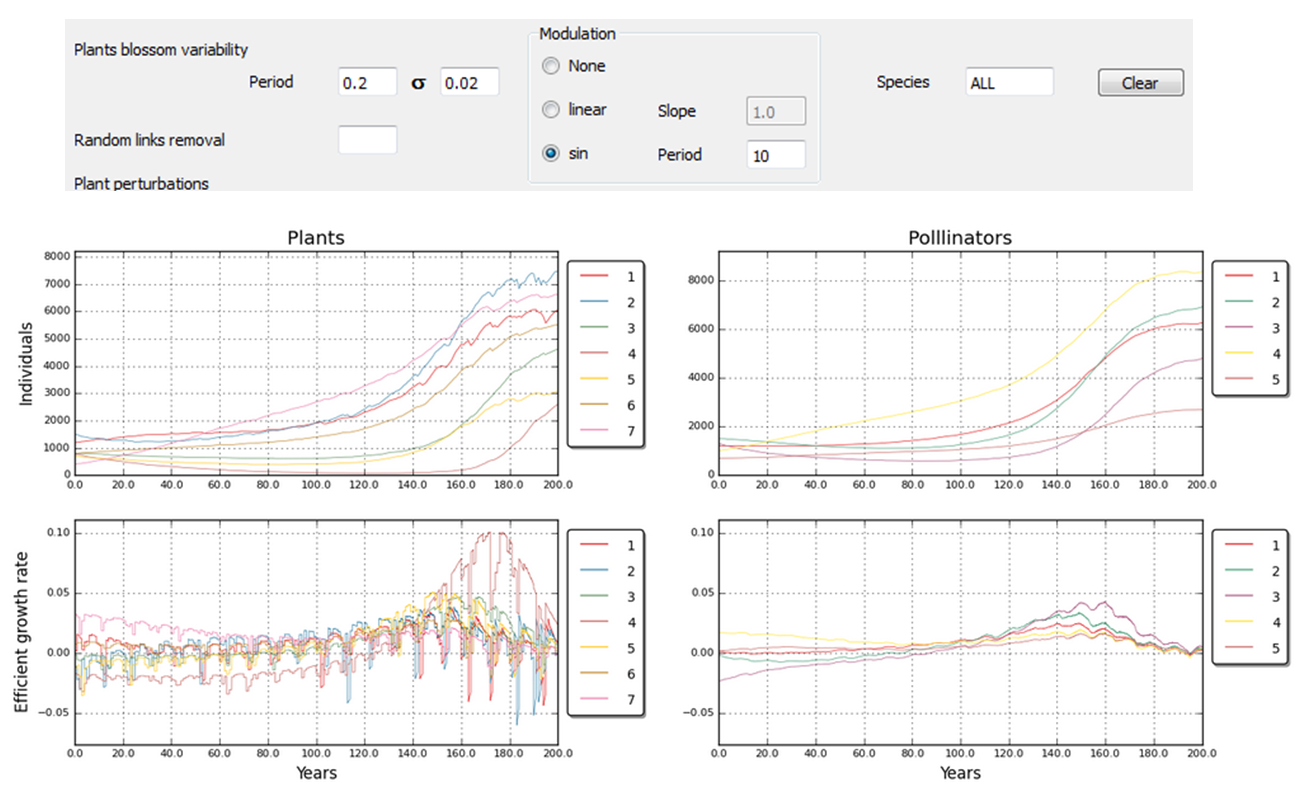
\includegraphics[scale=1]{ManFigs/sigmund_oscilacion_tiempo_sin.png}
\caption{Perturbación gaussiana en el periodo de floración con oscilación sinusoidal de la desviación estándar.}
\label{fig:ASIGMUNDMAN_sigmund_oscilacion_tiempo_sin}
\end{figure}

\begin{figure}[hp!]
\centering
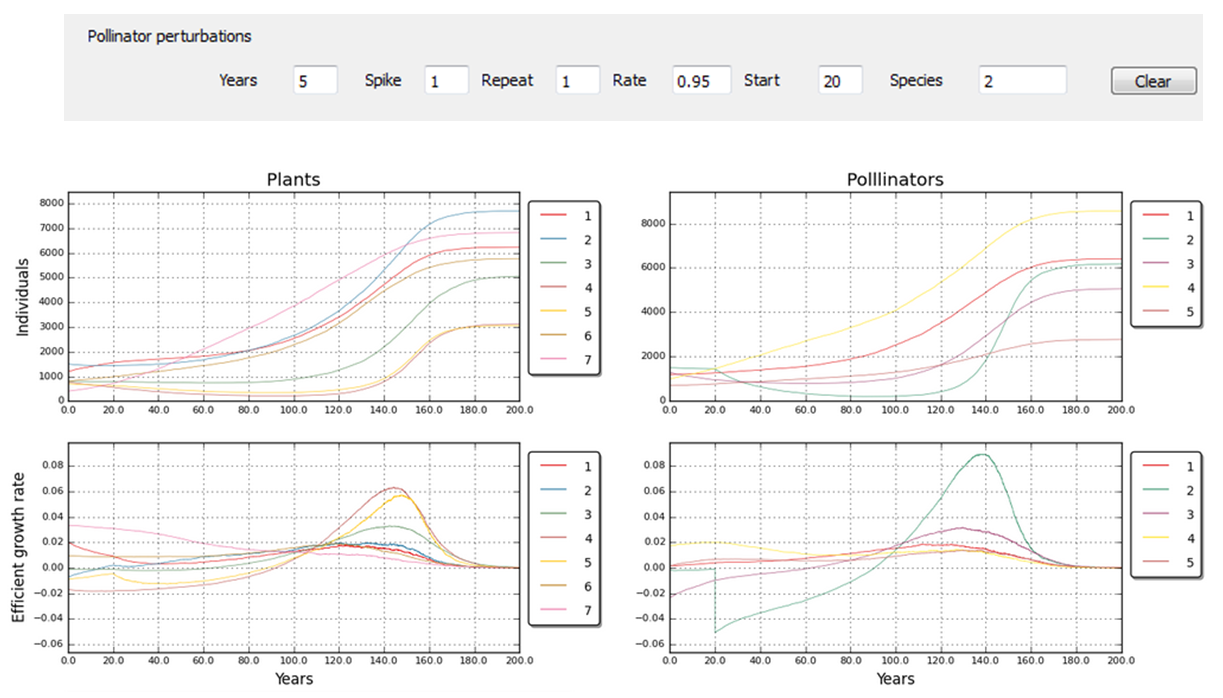
\includegraphics[scale=1]{ManFigs/sigmund_95.png}
\caption{Aumento abrupto de la mortalidad de la especie de polinizador número $2$.}
\label{fig:ASIGMUNDMAN_sigmund_95}
\end{figure}

Por el contrario, en la figura \ref{fig:ASIGMUNDMAN_sigmund_oscilacion_tiempo_sin}, la desviación estándar no es constante sino que oscila sinusoidalmente entre $0$ y $0.2$ según un periodo de 10 años. La red no se destruye como resultado de esta perturbación, simplemente tarda más en alcanzar los valores máximos de población. Aunque la amplitud de la oscilación crezca, la red se muestra mucho más resistente a los cambios cíclicos que cuando estos no ocurren en fase.

Para terminar estos ejemplos, se simulará el comportamiento de la red ante aumentos abruptos pero breves de la mortalidad. Este tipo de perturbaciones que actúan a corto plazo, a diferencia de las que se acaban de describir, pueden servir para modelar eventos como zoonosis, plagas o desastres naturales. El simulador permite atacar ambas clases con parámetros independientes para cada una.

En la figura \ref{fig:ASIGMUNDMAN_sigmund_95} se añade una mortalidad del $95\%$ durante $5$ años a la especie de polinizador $2$. La caída brusca está a punto de llevar a esta especie a la extinción pero al desaparecer, el beneficio mutualista hace que se recupere porque no baja del mínimo vital aunque llega a estar muy próxima a él alrededor del año $90$ de la simulación.

\section{Uso en modo \textit{batch}}

SIGMUND se puede lanzar en modo \textit{batch} desde la línea de comandos para realizar todo tipo de experimentos. El script se llama \texttt{sigmund\_standalone.py}. La simulación puede utilizar los parámetros almacenados en un fichero con una simulación previa, recibir
valores por línea de comandos o una combinación de ambas opciones.

\subsection{Configuración del script sigmund\_standalone.py}

\noindent Sintaxis de la llamada

\fontsize{3mm}{3mm}\selectfont
\begin{verbatim}
usage: sigmund_standalone.py [-h] [-simfile SIMFILE_NAME] [-g] [-v]
                             [-years SIM_YEARS] [-fw] [-outsf OUTSF] [-ds]
                             [-dsdir DSDIR] [-stop] [-rlink RLINK]
                             [-Blprob BLPROB] [-Blsd BLSD] [-Bltype BLTYPE]
                             [-Blspecies BLSPECIES] [-Bssvarper BSSVARPER]
                             [-Bssvarsd BSSVARSD] [-Bssvartype BSSVARTYPE]
                             [-Bssvartype_param BSSVARTYPE_PARAM]
                             [-Bssvarspecies BSSVARSPECIES]
                             [-pl_ext_period PL_EXT_PERIOD]
                             [-pl_ext_spike PL_EXT_SPIKE]
                             [-pl_ext_numperiod PL_EXT_NUMPERIOD]
                             [-pl_ext_rate PL_EXT_RATE]
                             [-pl_ext_start PL_EXT_START]
                             [-pl_ext_species PL_EXT_SPECIES]
                             [-pol_ext_period POL_EXT_PERIOD]
                             [-pol_ext_spike POL_EXT_SPIKE]
                             [-pol_ext_numperiod POL_EXT_NUMPERIOD]
                             [-pol_ext_rate POL_EXT_RATE]
                             [-pol_ext_start POL_EXT_START]
                             [-pol_ext_species POL_EXT_SPECIES]

optional arguments:
  -h, --help                           show this help message and exit
  -simfile SIMFILE_NAME                Simulation parameters file
  -g                                   Generate and store graphs
  -v                                   Verbose output
  -years SIM_YEARS                     Simulation span in years
  -fw                                  Superimposed food web
  -outsf OUTSF                         Append suffix to output file names
  -ds                                  Results data save
  -dsdir DSDIR                         Data save directory
  -stop                                On extinction stop simulation
  -rlink RLINK                         Randomlinks removal
  -Blprob BLPROB                       Blossom probability
  -Blsd BLSD                           Blossom deviation
  -Bltype BLTYPE                       Blossom type: Binary, Gaussian
  -Blspecies BLSPECIES                 Blossom species
  -Bssvarper BSSVARPER                 Blossom variability period
  -Bssvarsd BSSVARSD                   Blossom variability deviation
  -Bssvartype BSSVARTYPE 			   Blossom variability modulation type: None, linear, sin
  -Bssvartype_param BSSVARTYPE_PARAM   Blossom variability modulation parameter
  -Bssvarspecies BSSVARSPECIES 		   Blossom variability affected species
  -pl_ext_period PL_EXT_PERIOD         Plants external pert, period in years
  -pl_ext_spike PL_EXT_SPIKE           Plants external pert, spike (fraction of period)
  -pl_ext_numperiod PL_EXT_NUMPERIOD   Plants external pert, repeat pert
  -pl_ext_rate PL_EXT_RATE             Plants external pert, rate
  -pl_ext_start PL_EXT_START           Plants external pert, initial year
  -pl_ext_species PL_EXT_SPECIES       Plants external pert, affected species
  -pol_ext_period POL_EXT_PERIOD       Pollinators external pert, period in years
  -pol_ext_spike POL_EXT_SPIKE         Pollinators external pert, spike
  -pol_ext_numperiod POL_EXT_NUMPERIOD Pollinators external pert, repeat pert
  -pol_ext_rate POL_EXT_RATE           Pollinators external pert, rate
  -pol_ext_start POL_EXT_START         Pollinators external pert, initial year
  -pol_ext_species POL_EXT_SPECIES     Pollinators external pert, affected species
\end{verbatim}
\normalsize

Ejemplo de uso: 

\fontsize{3mm}{3mm}\selectfont
\begin{verbatim}
./sigmund_standalone.py -simfile exp18_Verhulst_oso_20.sim -y 50 -g -rlink 0.1 -v
\end{verbatim}
\normalsize

En este ejemplo se cargan las condiciones de simulación almacenadas en el fichero \texttt{exp18\_Verhulst\_oso\_20.sim}, se indica que la simulación dure 50 años, que se generen y almacenen los resultados gráficos, que se elimine un $10\%$ de enlaces y que la salida sea en modo \texttt{verbose}, como si se hubiera invocado desde la interfaz de usuario. Cuando en el comando de llamada se incluyen parámetros como en este ejemplo, tienen precedencia sobre la configuración que haya en el fichero. Así, esta simulación cubre un periodo de 50 años con independencia de que en el fichero se indique otra cifra.  

Si el flag \texttt{-v} no se activa, el programa se ejecuta en modo silencioso. Si el flag \texttt{-stop} está activo, el script devolverá tan solo las cadenas de caracteres \texttt{"SURVIVAL"} o \texttt{"EXTINCTION"}. Con esta opción se pueden lanzar múltiples simulaciones para comprobar si la red sobrevive bajo las condiciones especificadas. La simulación se detiene cuando el programa comprueba que el sistema está por debajo del mínimo vital y que no puede remontar.


\subsection{Script survival.py}

\noindent Este ejemplo muestra como puede usarse el script \texttt{sigmund\_standalone.py} cuando se elimina de forma aleatoria el $70\%$ de los enlaces de la red a lo largo de un periodo de 50 años.

\fontsize{3mm}{3mm}\selectfont
\begin{verbatim}
import subprocess
survival_success  =  0
no_experiments  =  50
com_base = "python3 sigmund_standalone.py -simfile exp18_10.sim -y 50 -stop -rlink 0.7"
for i in range(0,no_experiments):
    b = subprocess.check_output(com_base+str(rrate), shell=True)
    if str(b).find("EXTINCTION") == -1:
        print("remove links "+str(rrate)+" survival")
        survival_success += 1
    else:
        print("remove links "+str(rrate)+" extinction")
print("Experiments "+str(no_experiments)+"/ Network survived " \
      + str(survival_success)+" times")
\end{verbatim}
\normalsize

En este script se invoca \texttt{sigmund\_standalone.py} como un proceso externo, se puede obtener el mismo resultado con cualquier
otro lenguaje de programación.

\subsection{Script sigmund\_createinput\_atmax.py}

En numerosas ocasiones resulta conveniente comenzar la simulación con todas las poblaciones en máximos. El cálculo de este valor es
algebraicamente complicado, pero muy sencillo si se deja evolucionar libremente al sistema hasta que alcanza el punto de equilibrio.
Este script lanza una simulación y crea dos ficheros de entrada con los parámetros de los originales, excepto las poblaciones iniciales
que se sustituyen por los valores de población máxima. Estos ficheros tienen el nombre de los originales con el sufijo \texttt{MAX}.

\fontsize{3.5mm}{3.5mm}\selectfont
\begin{verbatim}
./sigmund_createinput_atmax.py -fichout
\end{verbatim}
\normalsize


\normalsize

